\subsection{Ablation Study}
\label{sec:exp-ablation}

In this section, we explore the contributions of the various components of our system.
%All ablation results in this section are evaluated on the on the validation set.

\noindent
\textbf{Feature Variations}

We first evaluate table linking results using different feature combinations.
As the results shown in \tabref{tab:ablation-features},
all features in our model make a positive contribution to the final accuracy.
%Both the mention and context feature directly represents the latent semantic association
%between the embedding of an individual mention
%(either from itself or from its neighborhoods)
%and the candidate entity.
The mention feature is the most important one, since it encodes
the most direct information between the mention and the target entity.
We observe that when using coherence feature only, a significant decrease in
accuracy takes place, largely due to the lack of dominant and direct 
semantic association between mention-entity pairs.
%We observe that Micro Accuracy drops when adopting these two features only,
%but it still outperforms other ablations,
Nevertheless, the coherence feature is complementary to the others,
as it aims at discovering the latent correlation in a global perspective,
modeling whether different candidate entities in one column 
are close to each other, for example, sharing the same (or similar) type,
even though no explicit type or category information is attached to the entity.
% it also shows that our coherence feature is able to extract the latent correlation
%between the target concepts, even though no explicit type or category information
%is attached to each candidate entity.

\begin{table}[ht]
 	\small
	\centering
	\caption{Ablation test on validation set.}
	\label{tab:ablation-features}
	\begin{tabular} {c|c|c}
        \hline
		Feature Combination &   Micro Acc.  & Decrease in Acc. (\%) \\
		\hline
		Mention Only           &   0.604    & 12.7 \\
		Context Only        &   0.576    & 16.7   \\
		Coherence Only      &   0.279    & 59.6     \\
		Mention + Context      &   0.652    & 5.78    \\
		\hline
		Full                &   0.692    & 0.00  \\
        \hline
	\end{tabular}
\end{table}


In the example in \figref{fig:chinesetable}, the mention 
``
%钢铁侠
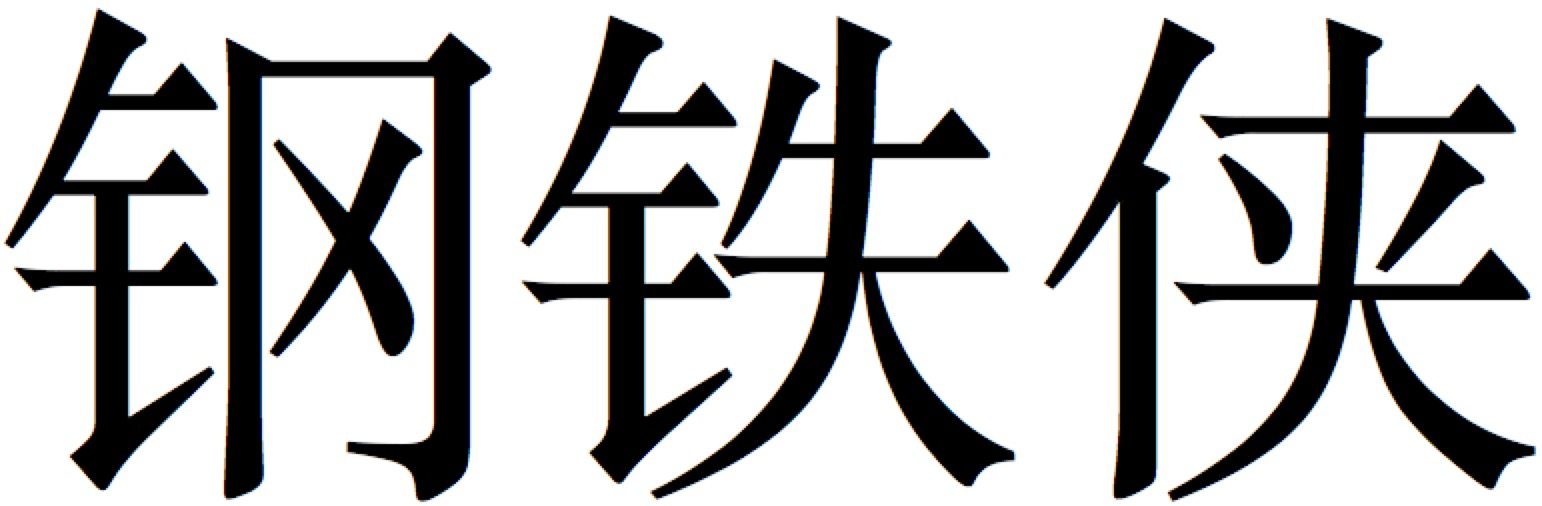
\includegraphics[height=1.3\fontcharht\font`\B]{figures/gangtiexia.png} 
'' can be linked to either
``Iron\_Man'' (the fictional superhero) or ``Iron\_Man\_(2008\_film)'' 
in Wikipedia, while both ``
%驯龙高手
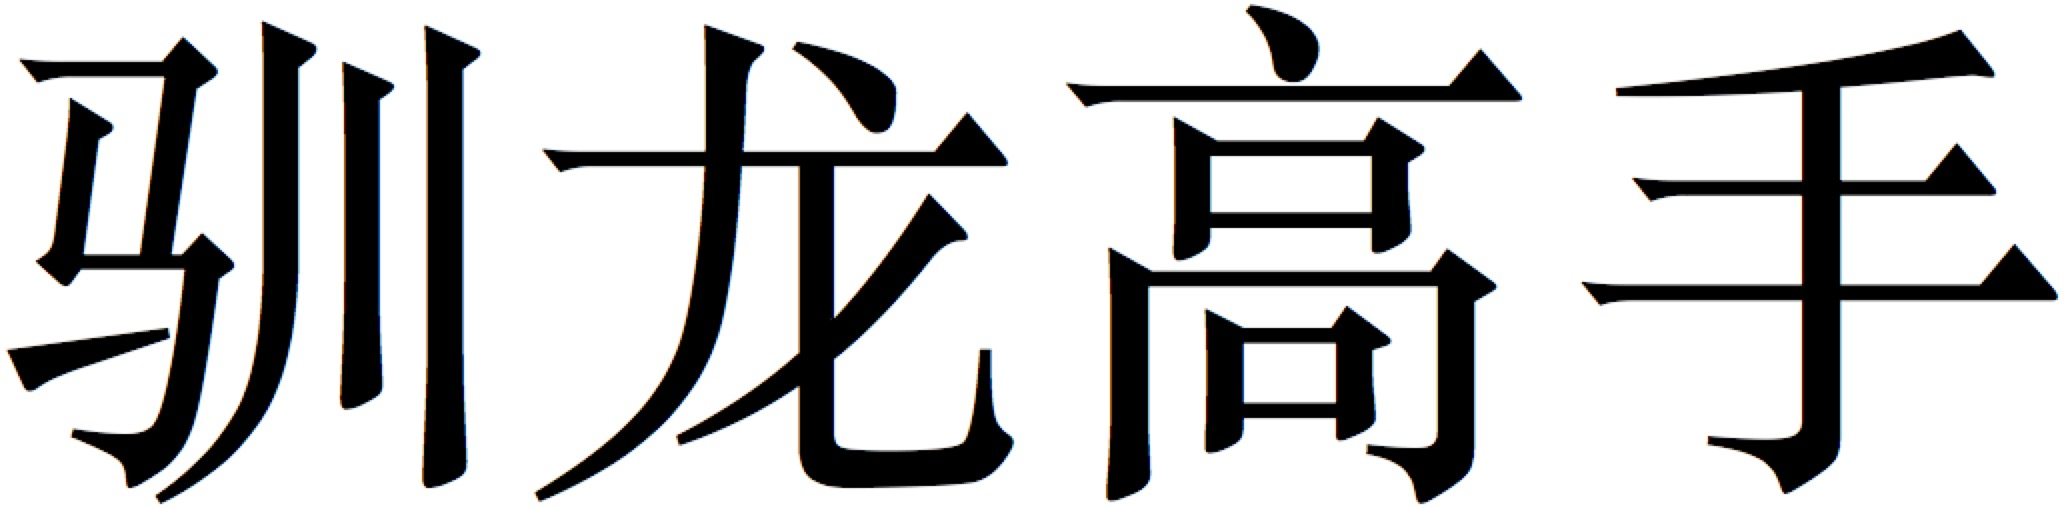
\includegraphics[height=1.3\fontcharht\font`\B]{figures/xunlong.png} 
'' (``How\_to\_Train\_Your\_Dragon\_(film)'') and
``
%线人
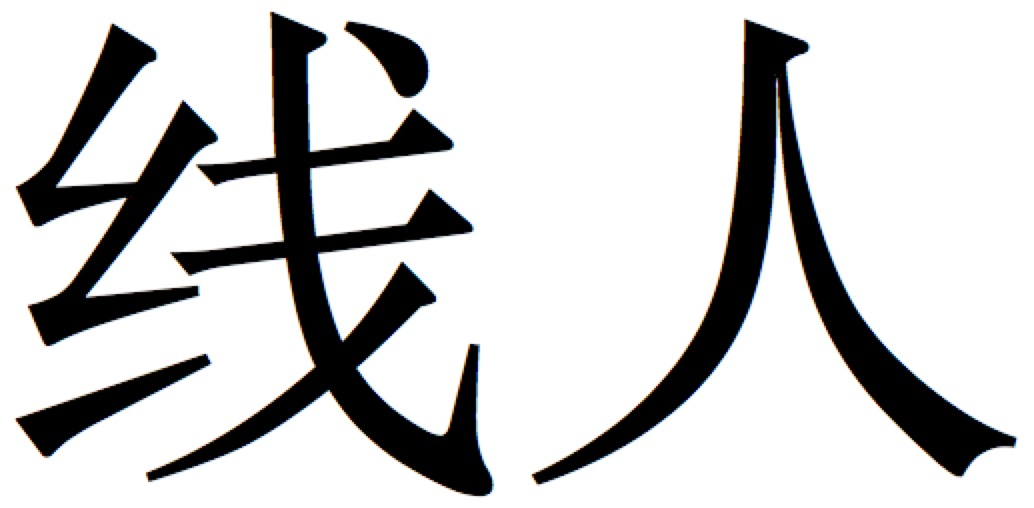
\includegraphics[height=1.3\fontcharht\font`\B]{figures/xianren.png} 
'' (``The\_Stool\_Pigeon\_(2010\_film)'') have less ambiguity.
Our model predicts the superhero when using mention + context features only.
After applying the coherence feature, 
the strong correlation between the entities in the same column
makes the model bias toward the correct film entity.


% \begin{figure}[th]
% \centering
% %\epsfig{file=fb-schema-4.eps, width=0.95\columnwidth}
% \scalebox{0.25}{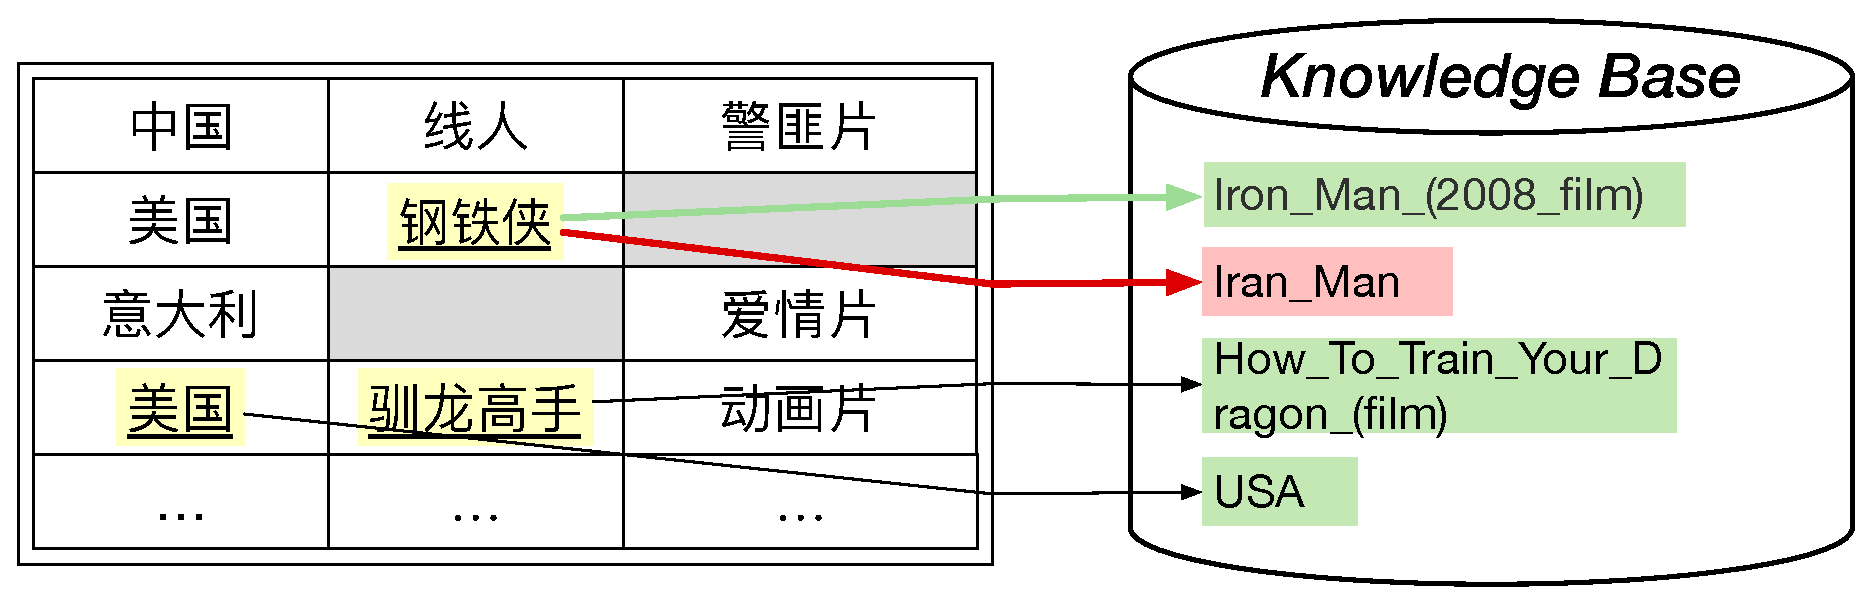
\includegraphics[angle=0]{figures/example.eps}}
% \caption{A real example of table linking. The red arrow points to the entity 
% predicted without using coherence feature, and the green arrow points to the entity
% predicted by using all features.}
% \label{fig:example}
% \end{figure}


\noindent
\textbf{Joint Model Versus Non-Joint Model}

Now we investigate the effectiveness of the joint framework.
%As discussed in \secref{sec:problem}, a non-joint model focus on 
%the scoring function between a single mention-entity pair.
Inspired by Sun et al.~\shortcite{sun2015modeling},
we change our joint scoring function back to the non-joint style,
where the the coherence module is removed,
and the average operation over different cells is no longer needed.
%Add formula if possible.
%Since there's no ranking information among single entities,
%to learn the parameters, we adopt hinge loss as the objective function,
%%RankNet is not available in the non-joint model 
%%due to no ranking information between single entities.
%%Therefore, we adopt hinge loss as the objective function,
%which maximizes the margin between the gold entity $e^+$ and
%all the negative entities $e^-$ of the mention $x$.
%We investigate the effect of joint model without introducing the coherence feature.
%As discussed before, the cell and context features focus on relationships of individual mentions,
%then we simply transform the table linking problem into a traditional entity linking problem.
%%:given a mention's cell and context embedding (rather than a table of multiple mentions),link the mention to an entity in the knowledge base.Also, the gold linking result of a training table becomes a list of $(mention, entity)$ pairs.
%
%Inspired by Sun et al. ~\shortcite{sun2015modeling}, we construct a non-joint model as the baseline: during training step, we adopt hinge loss as the optimizing function, 
%in order to maximize the margin $\lambda$ between the gold entity $e^+$
%and other entities $e^-$ of a mention $m$, defined as follows:
%\begin{equation}
%\label{eqn:hinge-loss}
%l_m = \max_{e^- \in Cand(m)} \max \{ 0, \lambda + score(m, e^-) - score(m, e^+) \}.
%%l_{m} = \max_{e^-}ffff
%\end{equation}
%
%\noindent
%In this model,  $score(\cdot, \cdot)$ is similar with \eqnref{eqn:score},
%but remove the coherence feature, and don't need to average cell and context features over mentions.
%The parameter $\lambda$ is tuned in \{1.0, 2.0, 3.0, 4.0\}.
As a comparision, we re-run our joint model but with the coherence module removed,
and use either hinge loss or RankNet as the optimizer.
%We also perform another ablation test, where we apply the joint model,
%but the pairwise rank loss is replaced by the hinge loss.
\tabref{tab:ablation-joint} shows Micro Accuracy results on the testing set.
We find that when using hinge loss, the non-joint model even 
outperforms the joint model.
We believe that hinge loss is less effective than RankNet in our joint model,
because: i) all the negative candidates of each mention are used in the 
non-joint model; however, in the joint model, 
some negative candidates are not sampled and hence cannot be observed by the model;
ii) hinge loss focuses on the margin between the positive entity table 
and the nearby negative entity table (with only a few corruptions),
thus other negative tables with more corruptions become less effective
in the training.
%As we can see, the RankNet based approach improves the Micro Accuracy by 0.024.
%Compared with the hinge loss, the RankNet method carries the intuition
%that the more corruption a table has, the lower score it holds.
%Once negative entity tables are comparable of each other, the training model
%could make full use of the training data.
It's worth mentioning that while the non-joint model is more 
light-weight at run time, the joint model takes only 6 rounds on average
for each prediction, which is acceptable in terms of running time.

\begin{table}[ht]
	\small
    \centering
    \caption{Micro-accuracies on the testing set under different model specifications.}
    \label{tab:ablation-joint}
    \begin{tabular} {c|c|c|c}
        \hline
        Model       & Optimizer     & Coherence  &  Micro Acc.   \\
        \hline
        Non-Joint   & Hinge Loss    & N     & 0.586         \\
        Joint       & Hinge Loss    & N     & 0.574         \\
        Joint       & RankNet       & N     & 0.598         \\
        Joint       & RankNet       & Y     & 0.629         \\
        %Joint (- coherence), Hinge Loss    &   0.574        \\
        %Joint (- coherence), RankNet         &   0.598      \\
        %Joint (+ coherence), RankNet         &   0.629     \\
        \hline
    \end{tabular}
\end{table}



%\textbf{Effect of pre-train data size.}
%Train on the common word dataset.
%Show experimental results, based on non-joint model.
%
%1) size of words, cosine similarity in test, final result
%
%2) or draw a figure, showing non-joint and joint accuracy trend.
%

